\section{Auswertung}
\label{sec:Auswertung}


Die Graphen wurden sowohl mit Matplotlib \cite{matplotlib} als auch NumPy \cite{numpy} erstellt. Die
Fehlerrechnung wurde mithilfe von Uncertainties \cite{uncertainties} durchgeführt.
Die Konstanten $k$, $\hslash$, $e_0$, $m_0$, $u_0$ und $N_\text{A}$ sind vom NIST \cite{nistgov}.

\subsection{Apparatekonstanten}
Der Ausgang "Oscillator" liefert eine konstante Spannung von $\SI{11,5}{\volt}$.
Am Ausgang "Reference" lässt sich die Spannung regeln.
\subsection{Ausgangssignal}
\subsubsection{Ausgangssignal ohne Rauschen}
\begin{figure}
\centering
\caption{Spannungsverläufe bei Phase $\Delta\phi$ ohne Tiefpassfilter}
\begin{minipage}{0.48\textwidth}
\center{$\Delta\phi=\SI{0}{\degree}$}
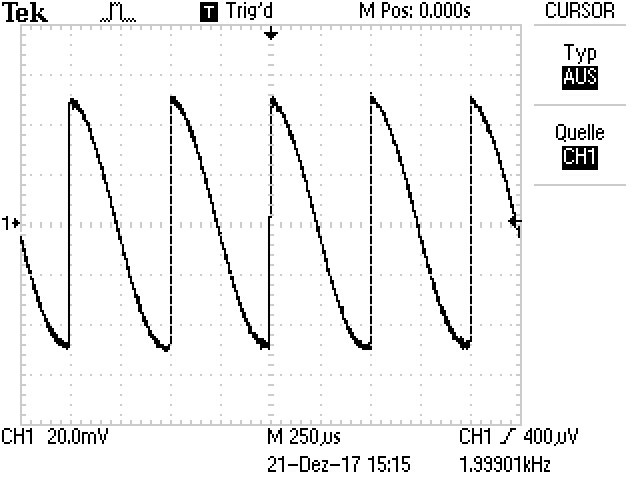
\includegraphics[scale=0.6]{content/images/00.jpg}
\end{minipage}
\begin{minipage}{0.48\textwidth}
\center{$\Delta\phi=\SI{45}{\degree}$}
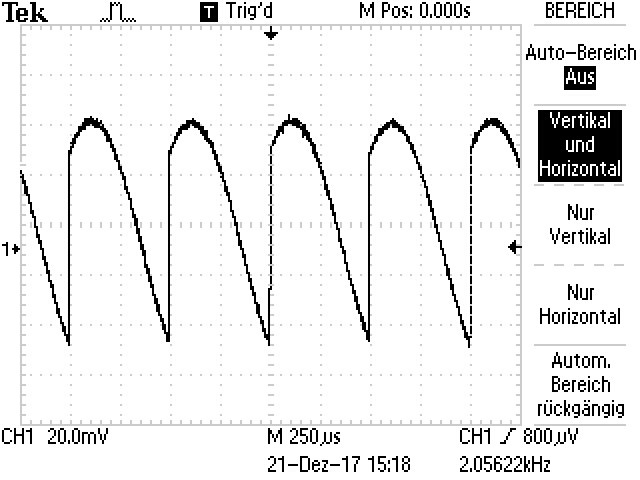
\includegraphics[scale=0.6]{content/images/45.jpg}
\end{minipage}
\begin{minipage}{0.48\textwidth}
\center{$\Delta\phi=\SI{90}{\degree}$}
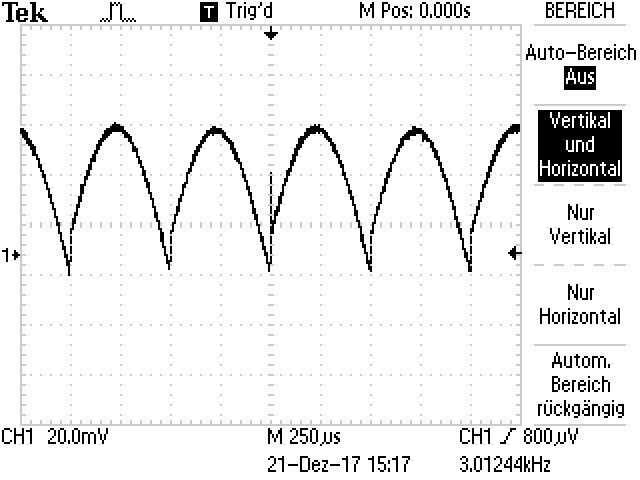
\includegraphics[scale=0.6]{content/images/90.jpg}
\end{minipage}
\begin{minipage}{0.48\textwidth}
\center{$\Delta\phi=\SI{180}{\degree}$}
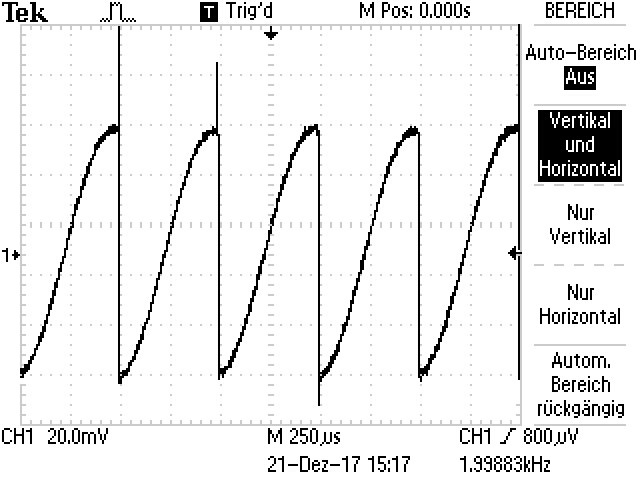
\includegraphics[scale=0.6]{content/images/180.jpg}
\end{minipage}
\center{$\Delta\phi=\SI{270}{\degree}$}
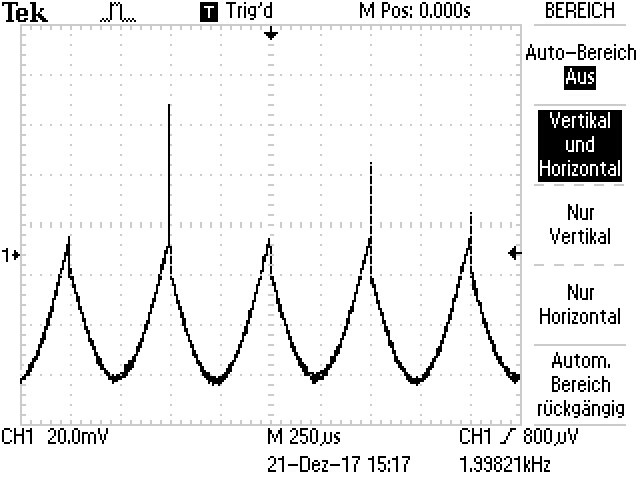
\includegraphics[scale=0.6]{content/images/270.jpg}
\label{fig:U}
\end{figure}
Die Spannung am "Reference"-Ausgang wurde auf $\SI{3,26}{\volt}$ bei $\SI{1000}{\hertz}$ eingestellt und der Gain des "Pre-Amplifier" auf 2 eingestellt. In Abbildung \ref{fig:U} sind die Spannungsverläufe für verschiedene Phasenverschiebungen $\Delta\phi$ abgebildet.
\begin{table}
	\centering
	\caption{Messwerte der Ausgangsspannung $U_.{out}$ nach dem Tiefpassfilter}
	\sisetup{table-format=1.2}
	\begin{tabular}{S[table-format=3.2] S[table-format=3.2]}
		\toprule
		{$T\phi/\si[per-mode=reciprocal]{\degree}$}&{$U_.{out}/\si[per-mode=reciprocal]{\volt}$ \\
		\midrule
		45 & 2,52 \\
		90 & 4,08 \\
		105 & 4,16 \\
		135 & 3,32 \\
		150 & 2,16 \\
		180 & 0,44 \\
		225 & -2,68 \\
		270 & -4,08 \\
		315 & -3,24 \\
		360 & -0,45 \\
		\bottomrule
	\end{tabular}
	\label{tab:tab1}
\end{table}
Mit den Messwerten mit eingeschaltetem Tiefpassfilter aus Tabelle \ref{tab:tab1} wird die Regression
$U_.{out}(\phi) = U_.{max}\cdot cos(f\cdot\phi+\phi_.0)$ durchgeführt:
\begin{align*}
U_.{max} &= \SI{4,13(5)}{\volt}
f 		 &= 17,5(1)e-3
\phi_.0  &= \SI{84(2)}{\degree}
\end{align*}
Mit Gleichung \eqref{eq:} ergibt sich für die Theoriekurve:
\begin{align*}
U_.{max,theo} &= \SI{4,15}{\volt}
f_.{theo}	  &= 17,5e-3
\phi_.{0,theo}&= \SI{0}{\degree}
\end{align*}
Damit ergibt sich eine Abweichung von den experimentellen zu den theoretischen Werten von:
\begin{align*}
\Delta U_.{max} &= 0,53\%
\Delta f		&= 0,00\%
\end{align*}
Die Graphen dazu sind in Abbildung \ref{fig:U2} zu sehen.
\begin{figure}
\centering
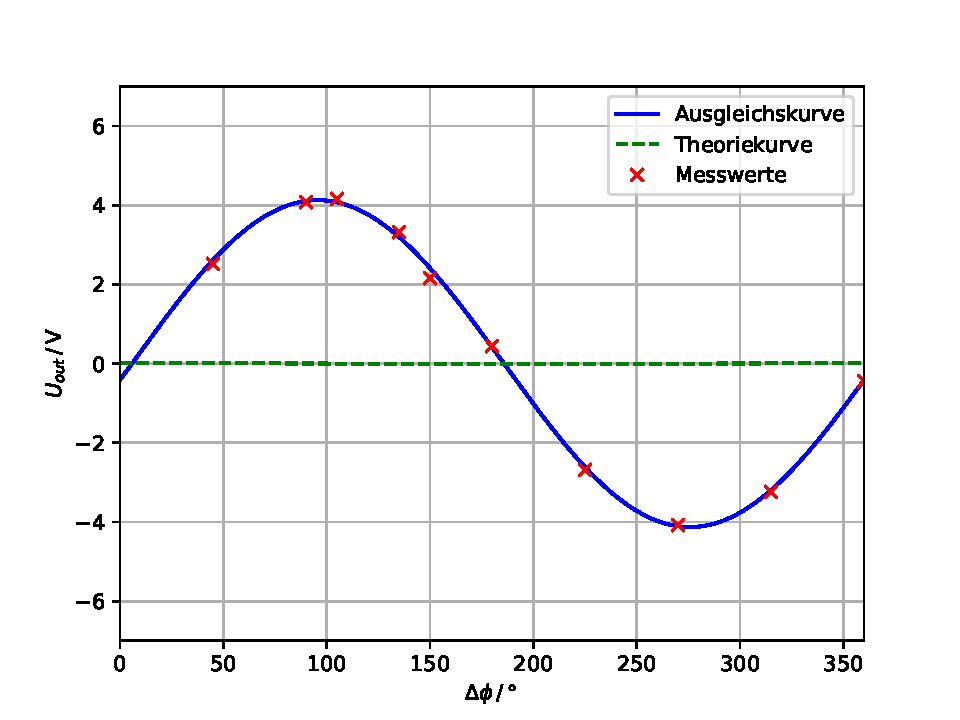
\includegraphics[scale=0.5]{content/images/plot.pdf}
\end{figure}
\subsubsection{Ausgangssignal mit Rauschen}